
\chapter[Các loại quang phổ]{Các loại quang phổ}
\section{Lý thuyết}
Mọi chất rắn, lỏng, khí được nung nóng đến nhiệt độ cao, đều phát ánh sáng. Quang phổ của ánh sáng do các chất đó phát ra gọi là quang phổ phát xạ của chúng.

\subsection{Quang phổ liên tục}

\begin{itemize}
	
	\item Là một dải có màu đỏ đến tím nối liền nhau một cách liên tục.
	
	\item Do các chất \textbf{rắn}, chất \textbf{lỏng} hoặc chất \textbf{khí} có áp suất lớn, phát ra khi bị nung nóng.
	
	\item Quang phổ liên tục của các chất khác nhau ở cùng một nhiệt độ thì \textbf{giống nhau} và \textbf{phụ thuộc vào nhiệt độ} của chúng.
	
\end{itemize}
\begin{center}
	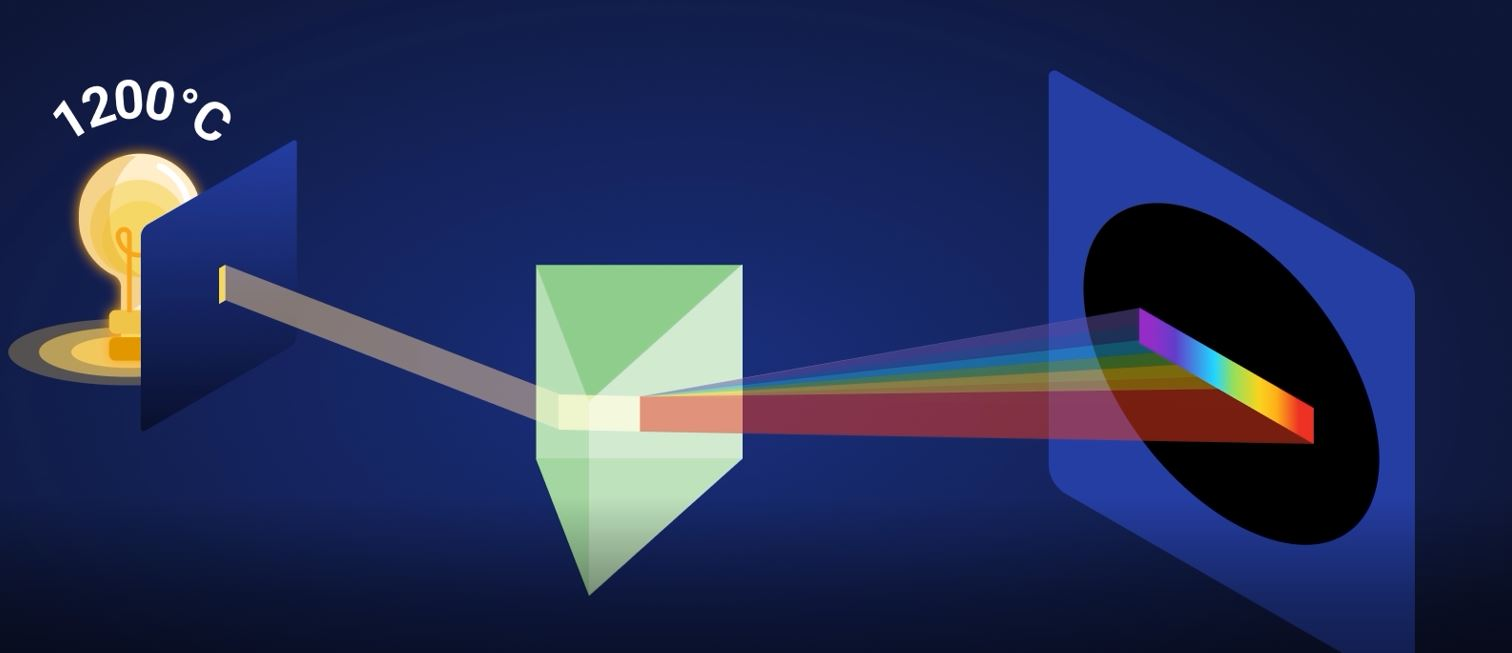
\includegraphics[width=10cm]{../figs/VN12-PH-36-L-021-2-1.JPG}
\end{center}

\subsection{Quang phổ vạch}

\begin{itemize}
	
	\item Là một hệ thống những \textbf{vạch sáng riêng lẻ}, ngăn cách nhau bởi những khoảng tối.
	
	\item Do chất \textbf{khí ở áp suất thấp} phát ra, khi bị kích thích bằng nhiệt hay bằng điện.
	
	\item Quang phổ vạch của các nguyên tố khác nhau thì \textbf{khác nhau} (số lượng các vạch, vị trí và độ sáng tỉ đối giữa các vạch).
	
	\item Mỗi nguyên tố hóa học có một quang phổ vạch đặc trưng của nguyên tố đó.
	
\end{itemize}

\begin{center}
	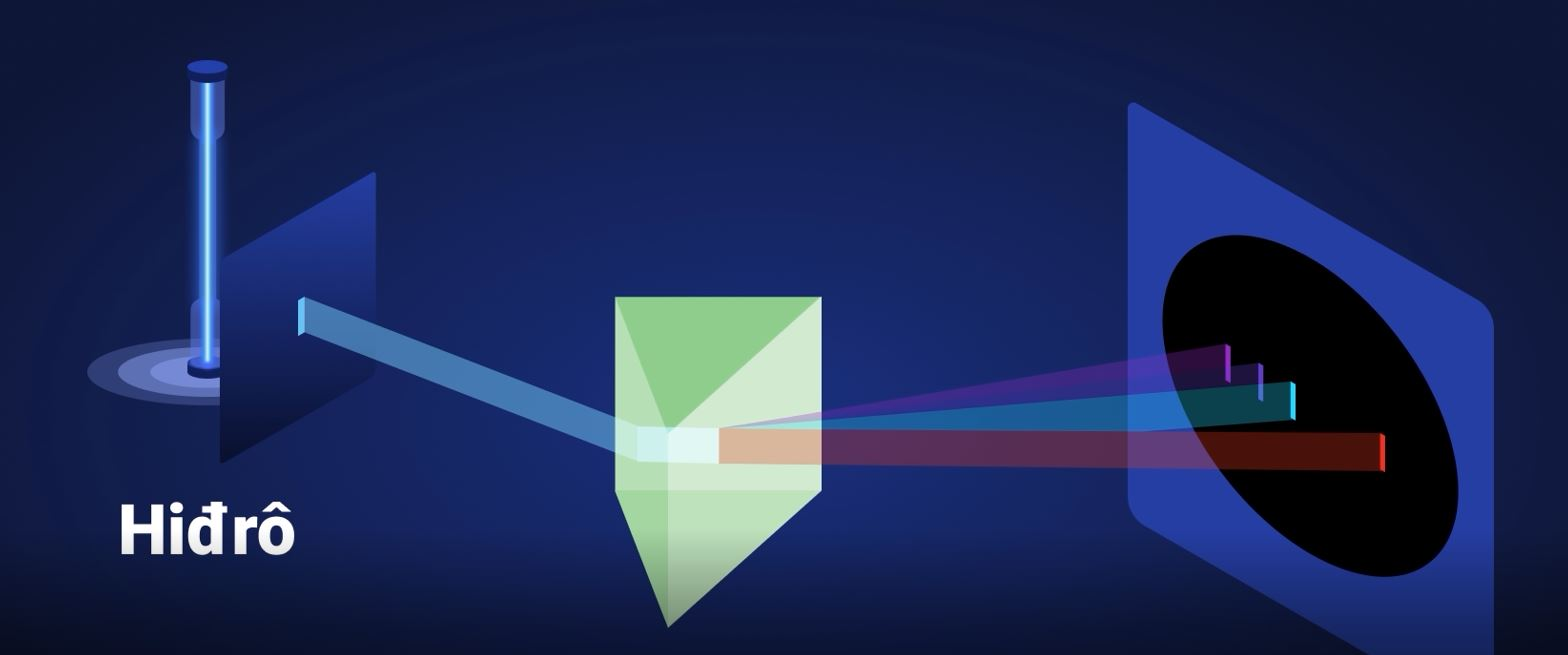
\includegraphics[width=10cm]{../figs/VN12-PH-36-L-021-2-2.JPG}
\end{center}

\subsubsection{Quang phổ hấp thụ}

\begin{itemize}
	
	\item Là các vạch hay đám vạch tối trên nền của một quang phổ liên tục.
	
	\item Điều kiện để thu được quang phổ hấp thụ là nhiệt độ của đám khí hay hơi hấp thụ phải thấp hơn nhiệt độ của nguồn sáng phát ra quang phổ liên tục.
	
	\item Sự đảo sắc vạch quang phổ là sự chuyển từ một vạch sáng trên nền tối thành vạch tối trên nền sáng, do bị hấp thụ.
\end{itemize}
\begin{center}
	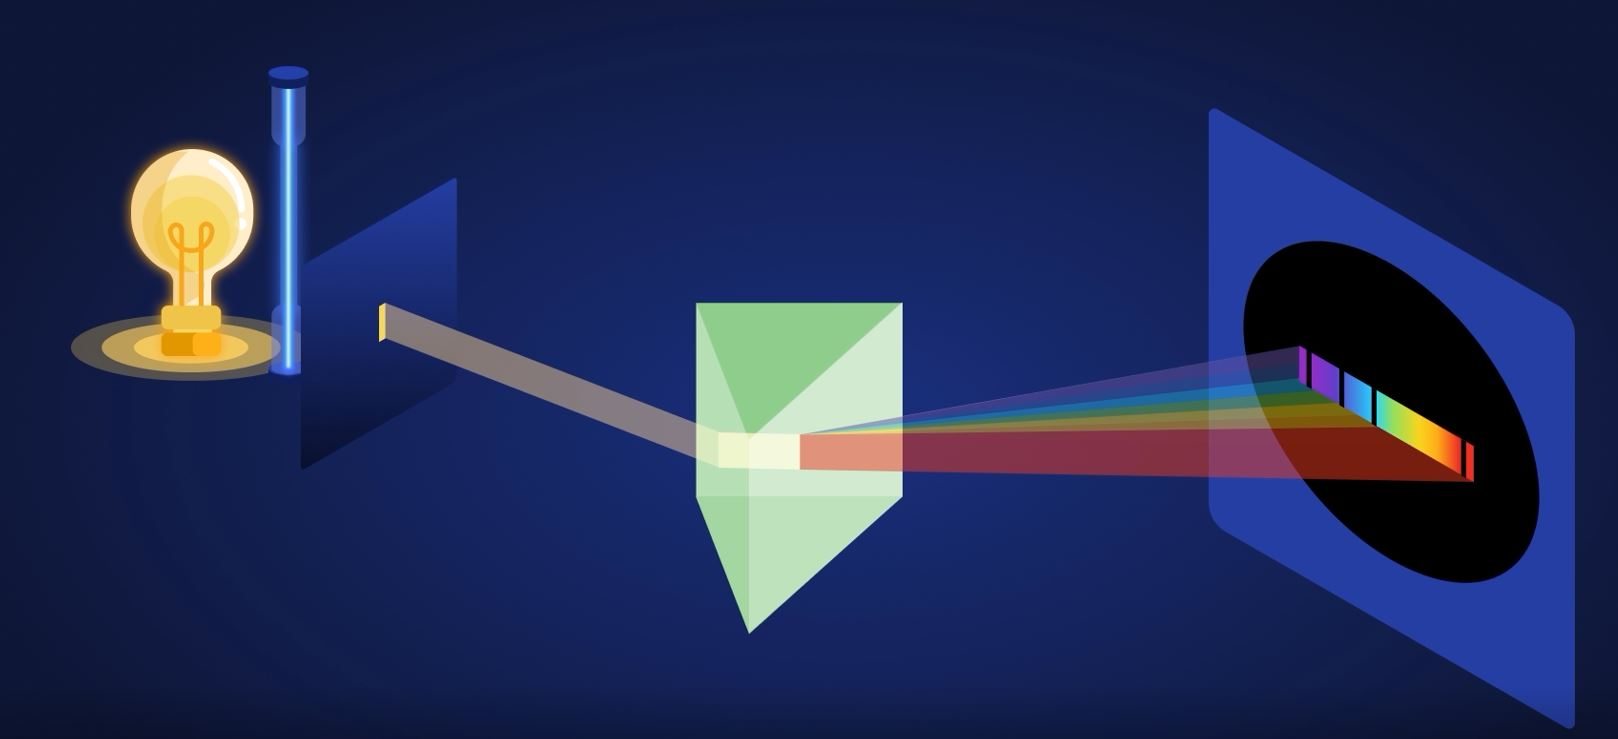
\includegraphics[width=10cm]{../figs/VN12-PH-36-L-021-2-3.JPG}
\end{center}
\luuy{Khí hay hơi có khả năng hấp thụ các vạch ở vị trí nào thì khi phát xạ cũng phát được các vạch sáng ở vị trí đó}
\section{Bài tập tự luyện}
\begin{enumerate}[label=\bfseries Câu \arabic*:]
	
	%========================================
	\item \mkstar{1} [2]
	\cauhoi
	{Quang phổ liên tục của một nguồn sáng phụ thuộc vào
		\begin{mcq}(1)
			\item nồng độ cấu tạo chất của nguồn sáng. 
			\item trạng thái cấu tạo của nguồn sáng. 
			\item nhiệt độ của nguồn sáng. 
			\item thành phần cấu tạo của nguồn sáng. 
		\end{mcq}
	}
	
	\loigiai
	{		\textbf{Đáp án: C.}
		
		Quang phổ liên tục của một nguồn sáng phụ thuộc vào thành phần cấu tạo của nguồn sáng. 
	}
	
	%========================================
	\item \mkstar{1} [3]
	\cauhoi
	{Để xác định nhiệt độ của một nguồn sáng ta dựa vào
		\begin{mcq}(2)
			\item quang phổ vạch. 
			\item quang phổ vạch phát xạ. 
			\item quang phổ vạch hấp thụ. 
			\item quang phổ liên tục. 
		\end{mcq}
	}
	
	\loigiai
	{		\textbf{Đáp án: D.}
		
		Để xác định nhiệt độ của một nguồn sáng ta dựa vào quang phổ liên tục. 
	}
	
	%========================================
	\item \mkstar{1} [12]
	\cauhoi
	{Quang phổ liên tục được phát ra khi nung nóng
		\begin{mcq}(1)
			\item chất rắn, chất lỏng, chất khí. 
			\item chất rắn, chất lỏng, chất khí có khối lượng riêng lớn. 
			\item chất rắn và chất lỏng. 
			\item chất rắn. 
		\end{mcq}
	}
	
	\loigiai
	{		\textbf{Đáp án: B.}
		
		Quang phổ liên tục được phát ra khi nung nóng chất rắn, chất lỏng, chất khí có khối lượng riêng lớn. 
	}
	
	%========================================
	\item \mkstar{1} [10]
	\cauhoi
	{Ứng dụng của việc khảo sát quang phổ liên tục là xác định
		\begin{mcq}(1)
			\item thành phần hóa học của một vật nào đó. 
			\item nhiệt độ và thành phần  cấu tạo hóa học của một vật nào đó. 
			\item hình dạng và cấu tạo của vật phát sáng. 
			\item nhiệt độ của các vật có nhiệt độ cao. 
		\end{mcq}
	}
	
	\loigiai
	{		\textbf{Đáp án: D.}
		
		Ứng dụng của việc khảo sát quang phổ liên tục là xác địnhnhiệt độ của các vật có nhiệt độ cao. 
	}
	
	%========================================
	\item \mkstar{1} [12]
	\cauhoi
	{Khi nói về quang phổ liên tục và quang phổ vạch phát xạ, phát biểu nào dưới đây \textbf{không} đúng? 
		\begin{mcq}(1)
			\item Quang phổ liên tục của các chất khác nhau nhưng ở cùng nhiệt độ thì hoàn toàn giống nhau. 
			\item Nguồn phát ra quang phổ vạch phát xạ là các chất khí có áp suất thấp khi bị kích thích. 
			\item Dựa vào quang phổ vạch phát xạ có thể xác định được thành phần cấu tạo của nguồn sáng. 
			\item Dựa vào quang phổ liên tục có thể xác định được thành phần cấu tạo của nguồn sáng. 
		\end{mcq}
	}
	
	\loigiai
	{		\textbf{Đáp án: D.}
		
		Không thể xác định được thành phần cấu tạo của nguồn sáng từ quang phổ liên tục.
	}
	
	%========================================
	\item \mkstar{1} [13]
	\cauhoi
	{Khi nói về quang phổ vạch phát xạ, phát biểu nào sau đây là \textbf{sai}?
		\begin{mcq}(1)
			\item Quang phổ vạch phát xạ của các nguyên tố hóa học khác nhau là khác nhau. 
			\item Hệ thống vạch phát xạ của một nguyên tố là hệ thống những vạch sáng riêng lẻ, ngăn cách nhau bằng những khoảng tối. 
			\item Trong quang phổ vạch phát xạ của hiđrô, ở vùng ánh sáng nhìn thấy có bốn vạch đặc trưng là đỏ, lam, chàm, tím. 
			\item Quang phổ vạch phát xạ phát ra do chất rắn và chất lỏng bị nung nóng.. 
		\end{mcq}
	}
	
	\loigiai
	{		\textbf{Đáp án: D.}
		
		Quang phổ phát ra do chất rắn và chất lỏng bị nung nóng là quang phổ liên tục.
	}
	
	%========================================
	\item \mkstar{1} [13]
	\cauhoi
	{Để thu được quang phổ vạch hấp thụ thì
		\begin{mcq}(1)
			\item nhiệt độ của đám khí hay hơi phải nhỏ hơn nhiệt độ của nguồn phát quang phổ liên tục. 
			\item Nhiệt độ của đám khí hay hơi phải lớn hơn nhiệt độ của nguồn phát quang phổ liên tục. 
			\item nhiệt độ của đám khí hay hơi hấp thụ phải lớn. 
			\item áp suất của đám khí hấp thụ phải lớn. 
		\end{mcq}
	}
	
	\loigiai
	{		\textbf{Đáp án: A.}
		
		Để thu được quang phổ vạch hấp thụ thì nhiệt độ của đám khí hay hơi phải nhỏ hơn nhiệt độ của nguồn phát quang phổ liên tục. 
	}
		\item \mkstar{1} 
	\cauhoi
	{Để nhận biết sự có mặt của nguyên tố hoá học trong một mẫu vật, ta phải nghiên cứu loại quang phổ nào của mẫu đó?
		
		\begin{mcq}(2)
			\item Quang phổ vạch phát xạ. 
			\item Quang phổ liên tục.
			\item Quang phổ hấp thụ. 	
			\item Cả ba loại quang phổ trên.
			
		\end{mcq}
	}
	
	\loigiai
	{		\textbf{Đáp án: A.}
		
	
	}
		\item \mkstar{1} 
	\cauhoi
	{Quang phổ của Mặt Trời mà ta thu được trên Trái Đất là
		
		\begin{mcq}(2)
			\item quang phổ liên tục. 	
			\item quang phổ vạch phát xạ.
			
			\item quang phổ vạch hấp thụ. 
			\item A, B, C đều đúng.
		\end{mcq}
	}
	
	\loigiai
	{		\textbf{Đáp án: C.}
		
		Quang phổ của ánh sáng Mặt Trời là quang phổ liên tục nhưng khi chiếu qua lớp khí quyển trên Trái Đất thì một số tia sáng đã bị hấp thụ.
	}
		\item \mkstar{2} 
	\cauhoi
	{Hiện tượng đảo sắc của vạch quang phổ (đảo vạch quang phổ) cho phép kết luận rằng
		
		\begin{mcq}(1)
			\item trong cùng một điều kiện về nhiệt độ và áp suất, mọi chất đều hấp thụ và bức xạ các ánh sáng có cùng bước sóng.
			
			\item ở nhiệt độ xác định, một chất chỉ hấp thụ những bức xạ nào mà nó có khả năng phát xạ và ngược lại, nó chỉ phát những bức xạ mà nó có khả năng hấp thụ.
			
			\item các vạch tối xuất hiện trên nền quang phổ liên tục là do giao thoa ánh sáng.
			
			\item trong cùng một điều kiện, một chất chỉ hấp thụ hoặc chỉ bức xạ ánh sáng.
			
		\end{mcq}
	}
	
	\loigiai
	{		\textbf{Đáp án: B.}
		
		Ở nhiệt độ xác định, một chất chỉ hấp thụ những bức xạ nào mà nó có khả năng phát xạ và ngược lại, nó chỉ phát những bức xạ mà nó có khả năng hấp thụ. 
	}
		\item \mkstar{2} 
	\cauhoi
	{Khẳng định nào sau đây là đúng?
		
		\begin{mcq}(1)
			\item  Vị trí vạch tối trong quang phổ hấp thụ của một nguyên tố trùng với vị trí vạch sáng màu trong quang phổ phát xạ của nguyên tố đó.
			\item Trong quang phổ vạch hấp thụ các vân tối cách đều nhau.
			
			\item Trong quang phổ vạch phát xạ các vân sáng và các vân tối cách đều nhau.
			
			\item Quang phổ vạch của các nguyên tố hoá học đều giống nhau ở cùng một nhiệt độ.
			
		\end{mcq}
	}
	
	\loigiai
	{		\textbf{Đáp án: A.}
		
		Vị trí vạch tối trong quang phổ hấp thụ của một nguyên tố trùng với vị trí vạch sáng màu trong quang phổ phát xạ của nguyên tố đó. 
	}
		\item \mkstar{1} 
	\cauhoi
	{Quang phổ của nguồn sáng nào sau đây không phải là quang phổ liên tục?
		
		\begin{mcq}(1)
			\item Sợi dây tóc nóng sáng trong bóng đèn. 
			\item Một đèn LED đỏ đang sáng.
			\item Mặt Trời. 	
			\item Miếng sắt nung nóng.
			
		\end{mcq}
	}
	
	\loigiai
	{		\textbf{Đáp án: B.}
		
		Đèn LED đỏ đang sáng là nguồn sáng đơn sắc. 
	}
\end{enumerate}

